\section{The sublinear range and a formula at every order}\label{sec:asymptotics}

The square-root correction is the first term of a convergent exponent. Retaining that exponent describes every sublinear order. Keeping the permutation denominator exact then gives one formula throughout the full range $2\le k\le N$.

Define, for $0\le t<1$,
\begin{equation}\label{eq:actionG}
G(t)=t+\frac{t^2}{2}+(1-t^2)\log(1-t)-\frac23t^3
=\sum_{j\ge4}\frac{2t^j}{j(j-2)}.
\end{equation}
All coefficients in the last series are positive.

\begin{theorem}[Uniform sublinear approximation]\label{thm:sublinear}
For every sequence $b_N=o(N)$ with $b_N\ge2$,
\begin{equation}\label{eq:sublinear}
\sup_{2\le k\le b_N}
\left|\frac{R_k}{H_k\exp\{NG(\sqrt{k/N})\}}-1\right|
\longrightarrow0.
\end{equation}
The supremum is over integers. The definition of $H_k$ remains \eqref{eq:hyperdef}, including $K=k-1$ at odd orders.
\end{theorem}

\begin{corollary}[Sharp thresholds for successive corrections]\label{cor:hierarchy}
For a fixed integer $p\ge4$, put
\[
G_p(t)=\sum_{j=4}^{p}\frac{2t^j}{j(j-2)}.
\]
Along any sequence $2\le k=o(N)$,
\begin{equation}\label{eq:hierarchy}
\frac{R_k}{H_ke^{NG_p(\sqrt{k/N})}}\longrightarrow1
\quad\Longleftrightarrow\quad
k=o\left(N^{(p-1)/(p+1)}\right).
\end{equation}
The ratio stays bounded exactly when $k^{p+1}/N^{p-1}$ stays bounded. At $k/N^{(p-1)/(p+1)}\to c\in(0,\infty)$ its limit is
\begin{equation}\label{eq:hierarchyboundary}
\exp\left(\frac{2c^{(p+1)/2}}{(p+1)(p-1)}\right).
\end{equation}
In particular, the correction $e^{k^2/(4N)}$ is relatively accurate up to $k=o(N^{3/5})$. Adding $2k^{5/2}/(15N^{3/2})$ to its exponent extends that range to $k=o(N^{2/3})$.
\end{corollary}

The thresholds in \eqref{eq:hierarchy} are uniform upper-range statements as well: the relative error tends uniformly to zero on $2\le k\le b_N$ whenever $b_N=o(N^{(p-1)/(p+1)})$. The conclusion concerns each fixed truncation degree $p$.

\subsection{A coefficient estimate with both angular peaks controlled}

Write
\[
f(z)=\frac{z}{1-z}+\log(1-z),\qquad
x=\sqrt{K/N},\qquad r=\frac{x}{1+x}.
\]
The positive saddle and its variance parameter are explicit:
\begin{equation}\label{eq:saddleequation}
Nrf'(r)=\frac{Nr^2}{(1-r)^2}=K,\qquad
b=N(r\partial_r)^2f(r)=2K(1+x).
\end{equation}

\begin{lemma}[Uniform positive-saddle estimate]\label{lem:saddle}
Let $2\le K\le N$ be integers, $\epsilon\in\{0,1\}$ and $K+\epsilon\le N$. Put $\lambda=(2/3)Nx^3$. There is an absolute constant $C$ such that
\begin{equation}\label{eq:saddlecoefficient}
[z^{K+\epsilon}]e^{Nf(z)}
=\frac{e^{Nf(r)}r^{-K-\epsilon}}{\sqrt{2\pi b}}(1+E),
\qquad |E|\le C\left(K^{-1}+e^{-\lambda/8}\right).
\end{equation}
The right side is a relative approximation when $K$ and $\lambda$ diverge. The bound remains valid without that divergence.
\end{lemma}
\begin{proof}
Cauchy's formula reduces the normalized coefficient to
\[
\frac1{2\pi}\int_{-\pi}^{\pi}
e^{\Phi(\theta)-i\epsilon\theta}\,d\theta,
\qquad
\Phi(\theta)=N(f(re^{i\theta})-f(r))-iK\theta.
\]
The positive coefficients of $f$ give
\begin{equation}\label{eq:angulardamping}
-\Re\Phi(\theta)
\ge Nr^2\sin^2\theta+\frac23Nr^3(1-\cos3\theta).
\end{equation}
Here $r\le1/2$ and $Nr^2=K/(1+x)^2\ge K/4$. On $|\theta|\le\pi/6$,
\[
\Re\Phi(\theta)\le-\frac9{4\pi^2}K\theta^2.
\]
For each fixed $q\ge2$, the derivative sum
\[
N\sum_{j\ge2}\frac{j-1}{j}j^qr^j
\le K\sum_{j\ge2}\frac{j-1}{j}j^q2^{2-j}
\]
is bounded by an absolute constant depending only on $q$, times $K$. Taylor's inequalities and \eqref{eq:saddleequation} therefore give
\[
\Re\Phi=-b\theta^2/2+O(K\theta^4),\qquad
|\Im\Phi|\le CK|\theta|^3.
\]
Pair conjugate angles. The central integrand becomes
$e^{\Re\Phi}\cos(\Im\Phi-\epsilon\theta)$. Using
$|\cos u-1|\le u^2/2$ and the real exponential mean-value bound, its difference from $e^{-b\theta^2/2}$ is at most
\[
C(K\theta^4+K^2\theta^6+\theta^2)e^{-cK\theta^2}.
\]
Its integral is $O(K^{-3/2})$, whereas the Gaussian integral is of order $K^{-1/2}$. The Gaussian tails outside the central interval are exponentially small.

The pair term alone does not suppress the other peak. Write $\theta=\pi+u$ modulo $2\pi$, with $|u|\le\pi/6$. Then
\[
1-\cos3\theta=1+\cos3u\ge1,\qquad
\frac23Nr^3=\frac\lambda{(1+x)^3}\ge\frac\lambda8.
\]
The pair term in \eqref{eq:angulardamping} supplies Gaussian decay in $u$. The second-peak integral is therefore at most $CK^{-1/2}e^{-\lambda/8}$. At the remaining angles, $|\sin\theta|\ge1/2$ and the integral is at most $Ce^{-K/16}$. Dividing by the central Gaussian integral proves \eqref{eq:saddlecoefficient}. The circle $r\le1/2$ stays away from the singularity at one, including at $K=N$.
\end{proof}

\subsection{Restoring parity and the permutation denominator}

For the moment normalization take $K=2\lfloor k/2\rfloor=2m$ and $\epsilon=k-K$. Set
\begin{equation}\label{eq:actionq}
h(x)=x+(x^2-1)\log(1+x)-\frac{x^2}{2},\qquad
q(x)=h(x)-\frac23x^3.
\end{equation}
The action identity is exact:
\[
Nf(r)-K\log r+K\log x-K/2=Nh(x).
\]
Stirling's formula applied to $m!$ in $\mathcal L_k$, followed by Lemma~\ref{lem:saddle}, gives
\begin{equation}\label{eq:normalizedsaddle}
\frac{Q_k}{\mathcal L_k}
=\frac{e^{Nh(x)}(1+x)^{\epsilon-1/2}}{2\lambda^\epsilon}
\left[1+O\left(K^{-1}+e^{-\lambda/8}\right)\right].
\end{equation}
Indeed, the even factorial cancellation leaves $2^mm!N^{-m}$ times the coefficient. At odd orders the additional factor is exactly
\[
\frac3{2Kr}=\frac{1+x}{\lambda}.
\]
Thus no odd-order shift is lost. The exact hyperbolic term is
$H_k=(e^\lambda+(-1)^\epsilon e^{-\lambda})/(2\lambda^\epsilon)$.
When $K$ and $\lambda$ exceed sufficiently large fixed constants, taking logarithms in \eqref{eq:normalizedsaddle} yields
\begin{equation}\label{eq:logsaddle}
\log\frac{R_k}{H_k}
=\log D_k+Nq(x)+(\epsilon-1/2)\log(1+x)
+O\left(K^{-1}+e^{-\lambda/8}\right).
\end{equation}

For the sublinear formula, put $t=\sqrt{k/N}$ and
$I(u)=u+(1-u)\log(1-u)$. Monotonicity of $-\log(1-v)$ bounds its left Riemann sum by
\begin{equation}\label{eq:denominatorintegral}
0\le NI(k/N)-\log D_k\le-\log(1-k/N).
\end{equation}
The derivative identities
$h'(x)=2x\log(1+x)$ and $q'(x)=2x(\log(1+x)-x)$ give $|q'(x)|\le x^3$. Since $t^2-x^2=\epsilon/N$,
$N|q(t)-q(x)|\le k/N$. Finally, $I(t^2)+q(t)=G(t)$ exactly. Hence, uniformly for $k/N\le1/16$ under the same large-$K$, large-$\lambda$ conditions,
\begin{equation}\label{eq:logsublinear}
\log\frac{R_k}{H_k}
=NG(\sqrt{k/N})+(\epsilon-1/2)\log(1+\sqrt{K/N})
+O\left(k/N+K^{-1}+e^{-\lambda/8}\right).
\end{equation}
The parity term has order $\sqrt{k/N}$ and must be retained for finer error estimates.

\begin{proof}[Proof of Theorem~\ref{thm:sublinear}]
On $\sqrt N<k\le b_N=o(N)$, the minimum $K$ is of order $\sqrt N$ and the minimum $\lambda$ is of order $N^{1/4}$. Every error in \eqref{eq:logsublinear}, and its explicit parity term, tends uniformly to zero. On $2\le k\le\sqrt N$, Theorem~\ref{thm:sqrt} applies, while the positive series \eqref{eq:actionG} gives
\[
0\le NG(\sqrt{k/N})-\frac{k^2}{4N}
\le C\frac{k^{5/2}}{N^{3/2}}\le CN^{-1/4}.
\]
This patches the two ranges and includes fixed orders. It does not assume a single-saddle relative approximation when $\lambda$ is small.
\end{proof}

\begin{proof}[Proof of Corollary~\ref{cor:hierarchy}]
For fixed $p$, positivity and decreasing coefficients give
\[
G(t)-G_p(t)=\frac{2t^{p+1}}{(p+1)(p-1)}(1+O_p(t))
\quad(t\to0).
\]
The first term bounds the tail from below, and the same term divided by $1-t$ bounds it from above. Theorem~\ref{thm:sublinear} therefore gives
\[
\log\frac{R_k}{H_ke^{NG_p(\sqrt{k/N})}}
=\frac{2k^{(p+1)/2}}{(p+1)(p-1)N^{(p-1)/2}}
\bigl(1+O_p(\sqrt{k/N})\bigr)+o(1).
\]
This proves relative accuracy, its necessity, boundedness and the boundary limit. The same positive-tail bound proves uniformity over the stated upper ranges. In particular,
\[
NG(\sqrt{k/N})
=\frac{k^2}{4N}+\frac{2k^{5/2}}{15N^{3/2}}
+\frac{k^3}{12N^2}+\frac{2k^{7/2}}{35N^{5/2}}+\cdots.
\]
The coefficient $2/15$ combines block weights, pair depletion and the permutation denominator. It is not the raw weight of a single five-element block.
\end{proof}

\subsection{Keeping the denominator exact}

For $2\le k\le N$, define
\begin{equation}\label{eq:globalformula}
\mathcal A_{N,k}
=D_kH_k e^{Nq(\sqrt{K/N})}
(1+\sqrt{K/N})^{\epsilon-1/2}.
\end{equation}
Every factor is positive and finite, including at $k=N$. Write
\[
\mathcal E_{N,k}=\frac{R_k}{\mathcal A_{N,k}}-1.
\]
The full exponent and the parity amplitude in \eqref{eq:globalformula} give a sharper global rate than the quartically corrected approximation considered in the next section. Its largest error occurs at cubic orders.

For $c>0$, put
\begin{equation}\label{eq:globalprofiledef}
\begin{gathered}
\ell(c)=\frac23c^{3/2},\qquad
p_0(t)=t\tanh t,\qquad p_1(t)=t\coth t-1,\\
\Phi_\epsilon(c)=\frac{3(2\epsilon-1)}{4c}
\bigl(p_\epsilon(\ell(c))-\ell(c)\bigr).
\end{gathered}
\end{equation}
Both profiles extend continuously to zero with value zero.

\begin{theorem}[Sharp uniform approximation at every order]\label{thm:global}
As $N\to\infty$,
\begin{equation}\label{eq:globalerror}
\sup_{2\le k\le N}|\mathcal E_{N,k}|
=C_*N^{-1/3}+o(N^{-1/3}),
\end{equation}
where the positive absolute constant is
\begin{equation}\label{eq:globalsharpconstant}
C_*=\max_{c>0}\frac3{4c}
\left(1-\frac{2\ell(c)}{e^{2\ell(c)}-1}\right).
\end{equation}
More precisely, the full-range parity profile satisfies
\begin{equation}\label{eq:globalprofile}
\sup_{2\le k\le N}
\left|N^{1/3}\mathcal E_{N,k}
-\Phi_{k\bmod2}(k/N^{1/3})\right|\longrightarrow0.
\end{equation}
Uniformly for $\sqrt N\le k\le N$, the error is
$O(K^{-1}+e^{-\lambda/8})$, and hence $O(N^{-1/2})$.

The maximum in \eqref{eq:globalsharpconstant} is attained at a unique $c_*>0$. If $z_*$ is the unique positive root of
\begin{equation}\label{eq:globalmaxequation}
2e^{2z}-(3z^2-z+4)e^z-z+2=0,
\end{equation}
then $c_*=(3z_*/4)^{2/3}$. Numerically,
\[
c_*\approx1.16540187318,\qquad C_*\approx0.395496270091.
\]
Odd orders nearest $c_*N^{1/3}$ attain the limiting supremum, with negative signed error. In particular, the exponent $1/3$ in \eqref{eq:globalerror} is optimal for \eqref{eq:globalformula}.
\end{theorem}
\begin{proof}
Appendix~\ref{sec:globalsharpproof} proves the compact critical expansion \eqref{eq:globalcompact}, retains both real saddle contributions, and controls both tails of $k/N^{1/3}$. These estimates give \eqref{eq:globalprofile}. The odd absolute profile strictly exceeds the even profile, and the appendix proves uniqueness of its maximizer, yielding \eqref{eq:globalerror} and \eqref{eq:globalsharpconstant}.

For the upper-range bound, divide \eqref{eq:normalizedsaddle} by the exact $H_k$. The residual factor is $(1+(-1)^\epsilon e^{-2\lambda})^{-1}$, which differs from one exponentially little for $k\ge\sqrt N$. The factor $D_k$ cancels exactly. This also explains why no approximation to $(N)_k$ is needed at $k=N$.
\end{proof}

At cubic orders, the four-block term and the common quadratic availability loss cancel between the moment and \eqref{eq:globalformula}. The remaining error records the difference between the mean shifted triple count $J-\epsilon$ and the Poisson parameter $\lambda$. The shift removes the compulsory triple at odd orders. Its contribution is divided by $K$, and its signs are opposite in the two parities. The uniform $N^{-1/4}$ rate in the next section concerns the different approximation $e^{k^2/(4N)}H_k$.

At the top order, Lemma~\ref{lem:saddle} can be used with degree $K=N$ and offset zero, without a parity restriction on that lemma. Here $r=1/2$ and $b=4N$, giving
\[
[z^N]e^{Nf(z)}=\frac{e^N}{\sqrt{8\pi N}}(1+O(N^{-1})),\qquad
a_N(N)=\frac{1+O(N^{-1})}{2N!}.
\]
This endpoint also follows from the classical truncated-exponential identity for $L_N^{(-N-1)}$. It is a consistency check on the full-range formula, rather than a separate priority claim.

\begin{figure}[htbp]
\centering
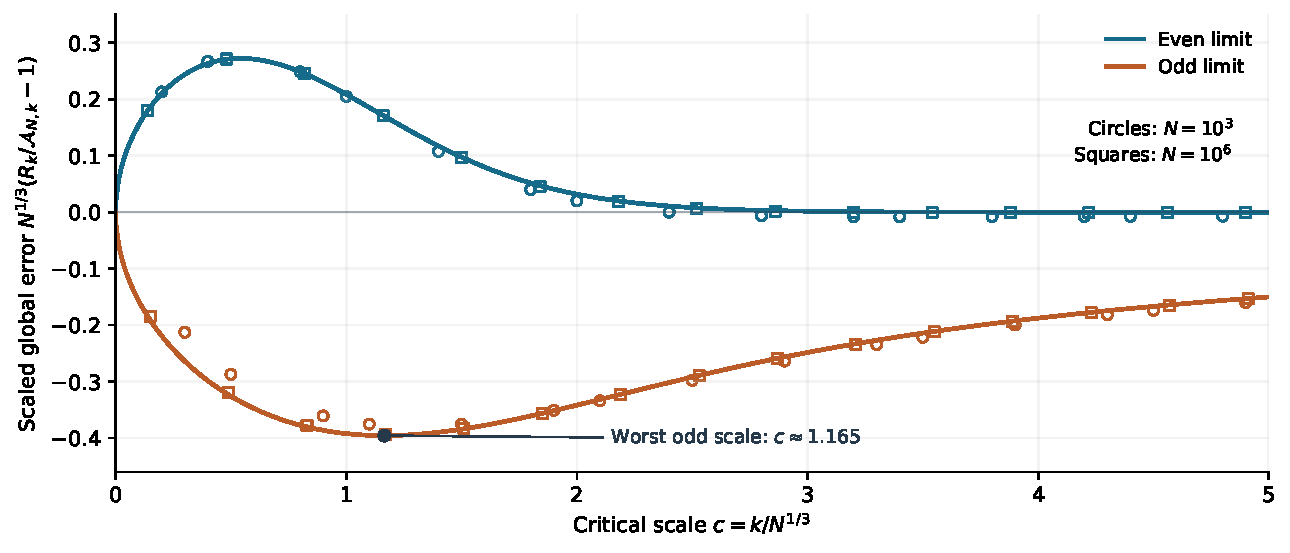
\includegraphics[width=.94\textwidth]{../figures/global-error.pdf}
\caption{The signed first error of the full-range approximation. The curves are the proved profiles in \eqref{eq:globalprofiledef}. Markers use the exact positive recurrence at $N=10^3$ and $N=10^6$. The odd profile has a unique minimum at $c_*\approx1.1654$, whose absolute value is $C_*\approx0.3955$. Finite values illustrate the limit and are not a substitute for its uniform proof.}
\label{fig:globalerror}
\end{figure}
